\documentclass[tikz,border=2pt]{standalone}
\usepackage{amsmath}
\usetikzlibrary{arrows.meta}
\begin{document}
% Precedence of & over | for x = 1..6. Left: (x<3) | ((x>4) & (x!=2)) keeps {1,2,5,6};
% right: ((x<3) | (x>4)) & (x!=2) keeps {1,5,6}. Each node is annotated with the values of x it keeps.
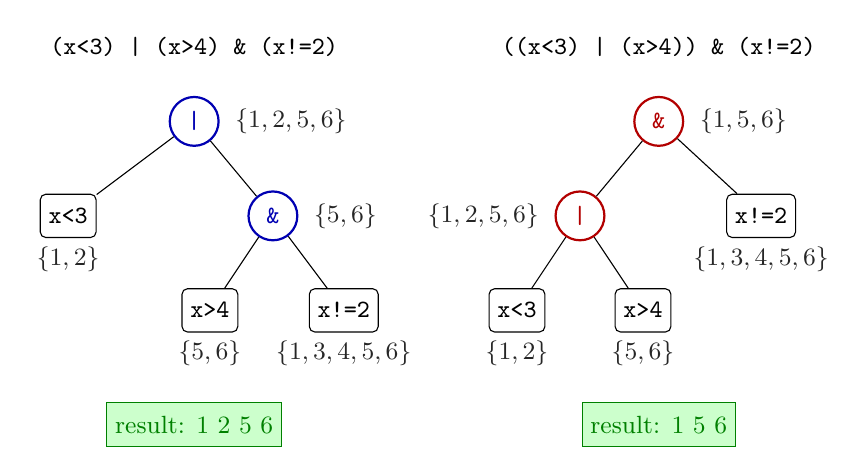
\begin{tikzpicture}[font=\small, >={Latex[length=2mm]},
  op/.style={circle, draw, thick, minimum size=0.62cm, inner sep=0pt, font=\small\ttfamily\bfseries},
  leaf/.style={draw, rounded corners=2pt, minimum height=0.55cm, inner sep=3pt, font=\small\ttfamily},
  keep/.style={gray!30!black, font=\small},
  res/.style={draw=green!50!black, fill=green!20, text=green!50!black, minimum height=0.55cm, inner sep=3pt}]
  % ---------- left: no extra parentheses ----------
  \begin{scope}
    \node[font=\small\ttfamily] at (2.4,1.35) {(x<3) | (x>4) \& (x!=2)};
    \node[op, blue!70!black] (r) at (2.4,0.4) {|};
    \node[keep, anchor=west] at (2.8,0.4) {$\{1,2,5,6\}$};
    \node[leaf] (a) at (0.8,-0.8) {x<3};
    \node[keep] at (0.8,-1.35) {$\{1,2\}$};
    \node[op, blue!70!black] (b) at (3.4,-0.8) {\&};
    \node[keep, anchor=west] at (3.8,-0.8) {$\{5,6\}$};
    \node[leaf] (c) at (2.6,-2.0) {x>4};
    \node[keep] at (2.6,-2.55) {$\{5,6\}$};
    \node[leaf] (d) at (4.3,-2.0) {x!=2};
    \node[keep] at (4.3,-2.55) {$\{1,3,4,5,6\}$};
    \draw (r) -- (a); \draw (r) -- (b); \draw (b) -- (c); \draw (b) -- (d);
    \node[res] at (2.4,-3.45) {result: 1 2 5 6};
  \end{scope}
  % ---------- right: parentheses around the | part ----------
  \begin{scope}[xshift=5.9cm]
    \node[font=\small\ttfamily] at (2.4,1.35) {((x<3) | (x>4)) \& (x!=2)};
    \node[op, red!70!black] (r) at (2.4,0.4) {\&};
    \node[keep, anchor=west] at (2.8,0.4) {$\{1,5,6\}$};
    \node[op, red!70!black] (b) at (1.4,-0.8) {|};
    \node[keep, anchor=east] at (1.0,-0.8) {$\{1,2,5,6\}$};
    \node[leaf] (d) at (3.7,-0.8) {x!=2};
    \node[keep] at (3.7,-1.35) {$\{1,3,4,5,6\}$};
    \node[leaf] (a) at (0.6,-2.0) {x<3};
    \node[keep] at (0.6,-2.55) {$\{1,2\}$};
    \node[leaf] (c) at (2.2,-2.0) {x>4};
    \node[keep] at (2.2,-2.55) {$\{5,6\}$};
    \draw (r) -- (b); \draw (r) -- (d); \draw (b) -- (a); \draw (b) -- (c);
    \node[res] at (2.4,-3.45) {result: 1 5 6};
  \end{scope}
\end{tikzpicture}
\end{document}
